\documentclass[xcolor=dvipsnames]{beamer}
\usepackage[utf8]{inputenc}

\usepackage{tikz}
\usetikzlibrary{positioning, calc}

%------------------------------------------------------------
%Theme
\usetheme{Madrid}
\usecolortheme[named=CadetBlue]{structure}
\setbeamertemplate{caption}[numbered]
\setbeamertemplate{bibliography item}[text]
%------------------------------------------------------------

%------------------------------------------------------------
%Title page
\title{Reinforcement Learning (DQN)}
\author{Pierre Squarra}
\date{Cognitive Algorithms Seminar}
%------------------------------------------------------------

\begin{document}

{
\logo{
\includegraphics[height=1cm]{tu-berlin}}
\begin{frame}
  \titlepage
\end{frame}
}

% Outline
\begin{frame}{Outline}
\tableofcontents
\end{frame}
%---------------------------------------------------------

\section{Reinforcement Learning}

\subsection{Key Concepts and Terminology}
\begin{frame}{Learning in Dynamic Environments}
    \begin{columns}
        \begin{column}{0.5\textwidth}
            \begin{figure}
                \centering
                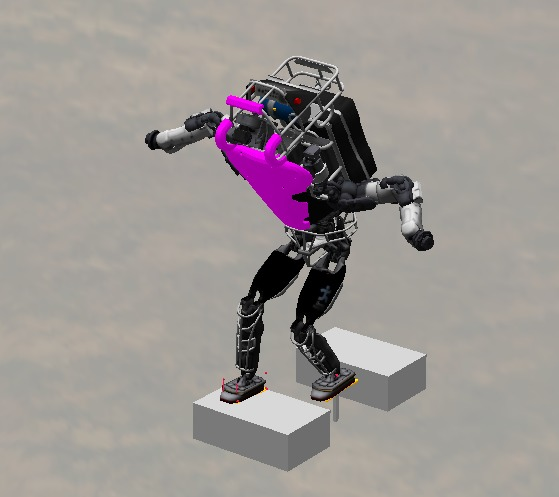
\includegraphics[height=0.8\textwidth]{atlas.jpg}
                \caption{Walking Robot \cite{wiedebach_walking_2016}}
                \label{fig:walking-robot}
            \end{figure}
        \end{column}
        \begin{column}{0.5\textwidth}
            \begin{figure}
                \centering
                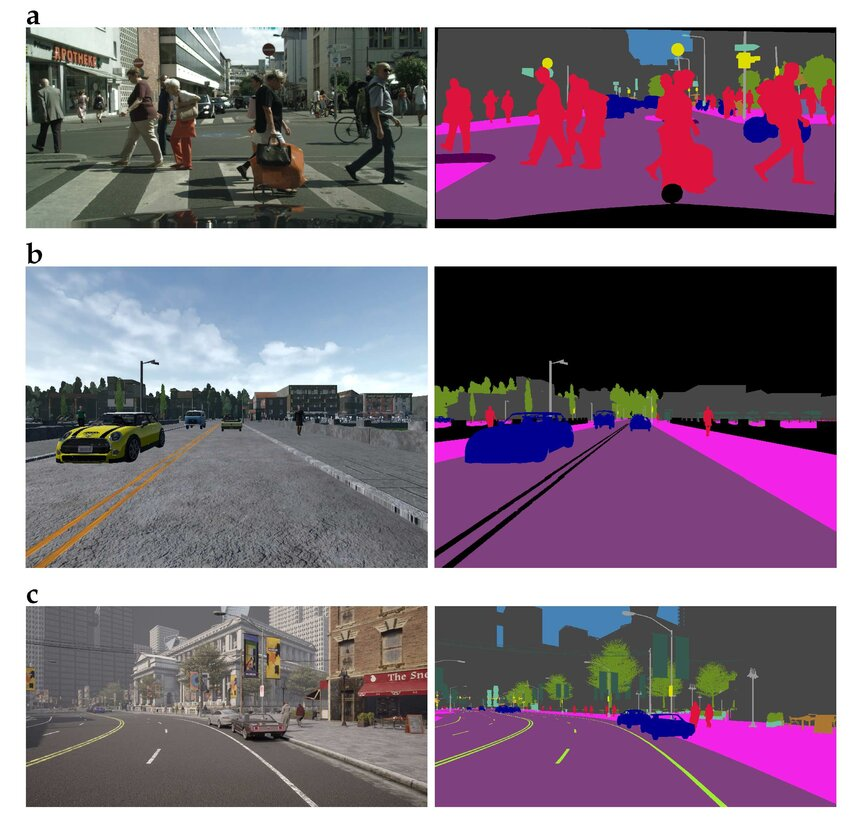
\includegraphics[height=0.8\textwidth]{tesla.jpg}
                \caption{Autonomous driving \cite{saha_practical_2023}}
                \label{fig:autonomous-driving}
            \end{figure}
        \end{column}
    \end{columns}
\end{frame}

\begin{frame}{Agent-Environment Interface}
    \begin{minipage}[c][2cm][c]{\textwidth}
        \only<1>{
            \textbf{Agent:} Decision-maker taking actions. \\
            \textbf{Environment:} World which the agent interacts with.
        }
        \only<2>{
            \textbf{Action:} Move the agent can make in the environment. \\
            \textbf{Observation:} Agent's perception of the environment.
        }
        \only<3>{
            \textbf{State:} Current situation or configuration of the environment. \\
            \textbf{Reward:} Scalar value measuring the success or failure of the agent's action.
        }
    \end{minipage}
    
    \tikzset{
    block/.style={rectangle, draw, text width=6em, text centered, minimum height=3em},
    action/.style={rectangle, color=white, fill=structure, text width=7em, text centered, minimum height=2em, rounded corners=5pt}}
    
    \begin{figure}
        \begin{tikzpicture}[very thick]
            % Nodes
            \node[block] (agent) {Agent};
            \node[block, right=5cm of agent] (environment) {Environment};
            \uncover<2->{\node[action, above=1cm of {$(agent)!0.5!(environment)$}] (actions) {Action};}
            \uncover<2->{\node[action, below=1cm of {$(agent)!0.5!(environment)$}] (observations) {Observation};}
            \uncover<3->{\node[below=0mm of actions] (action) {\small action $a_t$};}
            \uncover<3->{\node[above=0mm of observations] (new_state) {\small state $s_{t+1}$};}
            \uncover<3->{\node[below=0mm of observations] (reward) {\small reward $r_{t}$};}
            % Arrows
            \uncover<2->{\draw[-, color=structure] (agent.north) |- (actions.west);}
            \uncover<2->{\draw[->, color=structure] (actions.east) -| (environment);}
            \uncover<2->{\draw[-, color=structure] (environment.south) |- (observations.east);}
            \uncover<2->{\draw[->, color=structure] (observations.west) -| (agent.south);}
        \end{tikzpicture}
        \caption{The agent-environment interface \cite{sutton_reinforcement_2020}}
        \label{fig:agent-environment}
    \end{figure}
\end{frame}

\begin{frame}{Maze Example}
    \begin{columns}
        \begin{column}{0.5\textwidth}
            \begin{figure}
            \begin{tikzpicture}
                \filldraw[structure] (0.5,3.5) circle (0.2cm);
                \draw (3.5,4.5) node{-10};
                \fill[black] (2,2) rectangle (5,3);
                \fill[black] (2,1) rectangle (3,2);
                \draw (4.5,0.5) node{+10};
                \draw[step=1cm] (0,0) grid (5,5);
            \end{tikzpicture}
            \caption{Maze Example}
            \label{fig:maze-example}
            \end{figure}
        \end{column}
        \begin{column}{0.5\textwidth}
            \textbf{Agent:} 
            \begin{tikzpicture}[baseline=-0.5ex]
                \filldraw[structure] circle (0.2cm);
            \end{tikzpicture}
            
            \textbf{Actions:} $\{\boldsymbol{\uparrow}, \boldsymbol{\rightarrow}, \boldsymbol{\downarrow}, \boldsymbol{\leftarrow}\}$
            
            \textbf{States:} $\{(x, y) \mid x,y \in \{0, \dots, 4\}$
        \end{column}
    \end{columns}
\end{frame}

\begin{frame}{Returns and Value Functions}
    \begin{itemize}
        \item The agent’s job is to maximize cumulative reward, called the \alert{return}
        \begin{equation*}
            G_t = R_{t+1} + R_{t+2} + R_{t+3} + \dots
        \end{equation*}
        \begin{columns}
            \begin{column}{0.5\textwidth}
                \centering
                state-value function
                \begin{equation*}
                    v(s) = \mathbb{E} [G_t \mid S_t = s]
                \end{equation*}
                how good it is for the agent to be in a given state
            \end{column}
            \begin{column}{0.5\textwidth}
                \centering
                action-value-function
                \begin{equation*}
                    q(s,a) = \mathbb{E} [G_t \mid S_t = s, A_t = a]
                \end{equation*}
                how good it is to perform a certain action in a given state
            \end{column}
        \end{columns}
        \item We call the expected cumulative reward, from a state s, the \alert{value}
        \begin{equation*}
            v(s) = \mathbb{E} [G_t \mid S_t = s]
        \end{equation*}
        \item Goal is to \alert{maximize value}, by picking suitable actions
        \item It is also possible to condition the value on \alert{actions}
        \begin{equation*}
            q(s,a) = \mathbb{E} [G_t \mid S_t = s, A_t = a]
        \end{equation*}
    \end{itemize}
\end{frame}

\subsection{RL algorithms overview}
\subsection{Challenges in RL}

\section{Deep Q Networks}
\subsection{Workings of DQNs}
\subsection{Applications}

%---------------------------------------------------------
\begin{frame}[allowframebreaks]{References}
\bibliographystyle{ieeetr}
\bibliography{cognitive-algoritms-seminar}
\end{frame}

\end{document}